\documentclass[11pt]{article}

% ---------------------------------------------------------------------------
% Salience-Weighted Memory Retrieval for Long-Horizon Software Agents
% arXiv preprint source. Narrative synced to the public write-up; numbers and
% methodology drawn from the consolidated technical report (Experiments 1-5.1).
% Build: pdflatex main && bibtex main && pdflatex main && pdflatex main
% ---------------------------------------------------------------------------

\usepackage[utf8]{inputenc}
\usepackage[T1]{fontenc}
\usepackage{lmodern}
\usepackage[margin=1in]{geometry}
\usepackage{amsmath,amssymb}
\usepackage{booktabs}
\usepackage{graphicx}
\usepackage{array}
\usepackage{caption}
\usepackage{microtype}
\usepackage{enumitem}
\usepackage{xcolor}
\usepackage[hidelinks]{hyperref}
\usepackage{cleveref}

\graphicspath{{figures/}}

\newcommand{\sal}{\textsc{salience}}
\newcommand{\car}{\textsc{car}}

\title{\textbf{Salience-Weighted Memory Retrieval for Long-Horizon
Software Agents:\\ Retrieval Gains, Robustness, and an Honest Execution Null}}

\author{Alexander Julian Martinez\\
\small \href{https://github.com/alexanderjulianmartinez/mars}{github.com/alexanderjulianmartinez/mars}}

\date{June 2026}

\begin{document}
\maketitle

\begin{abstract}
A software agent that maintains a system over weeks accumulates a growing store of
memories --- design decisions, incident postmortems, naming conventions, and
documentation that slowly goes stale. It cannot fit all of this into a context window,
so a retrieval system must choose which memories to surface, and the standard choice
ranks every memory by semantic similarity to the current task. We study whether
augmenting similarity with computational \emph{salience} signals --- per-memory
\emph{importance} and \emph{confidence} --- improves retrieval quality, robustness, and
downstream agent behavior. We construct a frozen, hash-pinned, synthetic labeled
benchmark (30 queries, 552 memories, six adversarial categories) in which the most
semantically similar memories are deliberately distractors of low utility, defeating
similarity-only ranking. Across five studies on this single benchmark we find: (1)
importance-weighted retrieval improves recall@5 from $0.237$ to $0.672$ ($\Delta +0.435$)
and MRR from $0.313$ to $0.967$, with paired bootstrap confidence intervals that exclude
zero; (2) the advantage degrades gracefully and monotonically as importance is corrupted
toward random, never collapsing to the similarity baseline, with $\sim$78\% of the gain
attributable to the importance signal itself; (3) raw recency is \emph{not} a reliable
signal --- it helps only when artificially aligned with relevance, hurts symmetrically
when misaligned, and is statistically neutral in a realistic regime; (4) confidence
applied as a multiplicative gate on importance rescues a new ContradictionAvoidanceRate
from $0.000$ to $0.964$ when an important memory is wrong; and (5) in 18 real agent runs,
salience-aware retrieval improved retrieval and measurably changed the agent's behavior
(it adopted the repository's current convention over a stale one) but did \textbf{not}
raise task-success. We are explicit throughout that importance is authored and correlated
with relevance by construction (so the Experiment-1 effect is an upper bound), that the
benchmark is synthetic, and that retrieval gains do not by themselves imply agent
task-success gains. We position salience-weighted retrieval as a prioritization mechanism
for memory retrieval and report the execution result as an honest null.
\end{abstract}

% ===========================================================================
\section{Introduction}
% ===========================================================================

Agents that operate over long horizons --- across many turns, files, or sessions ---
accumulate memory. A coding agent maintaining a service over weeks records design
decisions, incident postmortems, naming and API conventions, and documentation that may
later become outdated. When the agent next acts, it cannot fit this entire history into a
context window, so a retrieval system selects a small subset to inject. The quality of
that selection bounds the quality of everything downstream.

The standard default is to rank candidate memories by semantic similarity to the current
task and treat the top-$K$ as interchangeable context. This default has a known failure
mode for long-horizon memory: the memory that is \emph{most similar} to a query is
frequently not the memory that is \emph{most useful}. Consider an agent adding
authentication to an endpoint whose memory contains two relevant items: a stale
\texttt{AUTH.md} describing the \emph{old} session-cookie scheme, and a buried postmortem
that says ``we migrated to JWT after the cookie incident.'' Semantic similarity loves the
stale doc --- it is full of auth vocabulary that matches the task --- while the
postmortem, written months ago in different words, ranks lower. Similarity surfaces the
wrong memory, the agent implements the deprecated approach, and the retrieval system never
had any way to express ``that note is out of date, and this decision matters more.''

That is the gap: similarity measures \emph{resemblance}, not \emph{usefulness}. We
investigate a narrow, practical hypothesis: \textbf{memories should not be treated as
equally important, and a retrieval ranker that incorporates salience signals beyond
similarity retrieves better.} ``Salience'' here is a deliberately computational notion ---
not an attempt to model emotion or affect, but a set of cognitive-style scalar signals
(importance, confidence, novelty, urgency, recency) that a memory system can attach to a
record and a ranker can consume. We isolate \textbf{importance} as the primary signal,
\textbf{confidence} as a gating signal, and treat \textbf{recency} as a candidate signal
that we test and ultimately reject.

This paper consolidates a five-experiment program in which each experiment after the first
probes a specific weakness of the result before it: the authored importance labels
(\cref{sec:exp2}), the role of time (\cref{sec:exp3}), the case where an important memory
is wrong (\cref{sec:exp4}), and whether any of it reaches a real agent (\cref{sec:exp5}).

\begin{quote}
Importance helps retrieval (\cref{sec:exp1}) $\to$ and survives noise (\cref{sec:exp2})
$\to$ recency does not earn a place (\cref{sec:exp3}) $\to$ confidence rescues
contradictions (\cref{sec:exp4}) $\to$ and inside a real agent, retrieval and behavior
change but task-success does not (\cref{sec:exp5}).
\end{quote}

\paragraph{Contributions.}
\begin{enumerate}[leftmargin=1.4em,itemsep=2pt]
\item \textbf{Salience Memory Benchmark v1.0.0} --- a frozen, hash-pinned synthetic
retrieval benchmark (30 queries, 552 memories, six labeled categories) engineered so that
similarity-only ranking is actively misled by high-overlap, low-importance distractors. It
is non-saturating, unlike the 13-memory smoke test it replaces, which scored recall@5
$=1.0$ for every strategy.
\item \textbf{Importance-weighted retrieval evaluation} --- a controlled, paired comparison
of salience-weighted vs.\ similarity-only retrieval over a real semantic backend (Cortex,
Voyage embeddings), with a full retrieval metric suite and paired bootstrap significance
testing (Experiment 1).
\item \textbf{Robustness analysis under noisy importance} --- a quality sweep showing the
advantage degrades gracefully and monotonically, attributing $\sim$78\% of the gain to the
importance signal itself (Experiment 2).
\item \textbf{Temporal salience ablation} --- an isolation of the recency term across four
timestamp regimes, finding recency unreliable as a primary signal (Experiment 3).
\item \textbf{Confidence-gated contradiction handling} --- a new ContradictionAvoidanceRate
metric and a gated $\mathrm{importance}\times\mathrm{confidence}$ formulation that prevents
important-but-wrong retrieval (Experiment 4).
\item \textbf{An honest real-agent execution study} --- an evidential 3-arm study (18 real
agent runs) that separates \emph{retrieval improved + behavior changed} from
\emph{task-success improved}, finding the former but not the latter (Experiments 5 and 5.1).
\end{enumerate}

The gap between contribution 6's two halves --- ``the agent retrieved better'' and ``the
agent did better'' --- is the organizing concern of this paper. Retrieval quality is a
proxy; task-success is the outcome; on our execution benchmark the two came apart, and we
keep that line sharp throughout.

% ===========================================================================
\section{Related Work}
% ===========================================================================

\paragraph{Retrieval-augmented generation (RAG).} A large body of work injects retrieved
text into a language model's context to ground its outputs~\cite{lewis2020rag}. The
dominant ranking signal is embedding similarity~\cite{karpukhin2020dpr}, optionally
combined with lexical scores in hybrid rankers. Our work is in this family but asks an
orthogonal question: rather than improving the \emph{similarity} estimate, we add a
\emph{non-similarity} per-memory signal (importance, then confidence) to the ranker. We do
not claim hybrid sparse/dense retrieval as novel; we claim that an authored salience term
is a distinct axis.

\paragraph{Agent memory systems.} Recent agent architectures maintain external memory
stores with summarization, reflection, and read/write policies, and several assign scalar
scores to memories (e.g.\ recency- and importance-style weights) when deciding what to
surface~\cite{park2023generative,packer2023memgpt}. Our contribution relative to this line
is not the idea that memories can carry an importance score, but a controlled, adversarial,
significance-tested \emph{evaluation} of that idea against a real semantic baseline,
together with an honest accounting of the authored-importance ceiling and an explicit
recency ablation.

\paragraph{Learning-to-rank and re-ranking.} Classical learning-to-rank~\cite{liu2009ltr}
and neural re-rankers~\cite{nogueira2020monot5} optimize ranking against graded relevance.
Our salience terms are closer to hand-specified priors than learned re-rankers; we
deliberately do not learn importance or confidence in this work, and we flag learned
estimation as the key open problem for real-world applicability.

\paragraph{Long-context models.} An alternative to selective retrieval is to expand the
context window and attend over more history. This trades retrieval precision for attention
cost and is complementary to ranking: even with a long window, inclusion and ordering
decisions affect what the model attends to~\cite{liu2024lostinthemiddle}. We do not
evaluate long-context baselines.

\paragraph{Attention as prioritization.} We use ``attention allocation'' informally to
mean \emph{which memories a system spends its limited context budget on}. We make no claim
about neural attention mechanisms inside the model, and we avoid any cognitive or affective
interpretation beyond the engineering one: salience is a prioritization prior over a memory
store.

We are cautious about novelty. The constituent ideas --- similarity ranking, scalar memory
importance, adversarial retrieval benchmarks --- exist. What we offer is a clean, frozen,
significance-tested measurement of importance and confidence under controlled conditions,
with ceiling effects made explicit, plus an honest execution null.

% ===========================================================================
\section{Salience-Weighted Retrieval}
\label{sec:method}
% ===========================================================================

\subsection{Setup and notation}
For a query $q$ and a candidate memory $m$ from the per-query retrieved pool, a ranking
strategy assigns a scalar score $s(q, m)$; memories are returned in descending score order
and the top-$K$ are evaluated. All strategies re-rank the \emph{same} retrieved pool, so
the comparison isolates the ranking function, not first-stage embedding recall.

Each memory carries: $\mathrm{sim}(q, m)\in[0,1]$ (semantic similarity from the embedding
backend), $\mathrm{imp}(m)\in[0,1]$ (authored importance), $\mathrm{conf}(m)\in[0,1]$
(authored confidence), $\mathrm{rec}(m)\in[0,1]$ (recency from write time), and
$\mathrm{freq}(m)\in[0,1]$ (access frequency). The benchmark also labels novelty and
urgency, which are not consumed by the strategies evaluated here.

\subsection{Baseline: similarity-only}
\begin{equation}
s_{\mathrm{sim}}(q, m) = \mathrm{sim}(q, m).
\end{equation}
This is the standard RAG ranker and the control condition.

\subsection{Candidate: salience-weighted (v1)}
\begin{equation}
s_{\mathrm{sal}}(q, m) = w_s\,\mathrm{sim}(q,m) + w_i\,\mathrm{imp}(m)
    + w_r\,\mathrm{rec}(m) + w_f\,\mathrm{freq}(m),
\end{equation}
with non-negative weights normalized to sum to 1. We use the default
$(w_s, w_i, w_r, w_f) = (0.40, 0.30, 0.20, 0.10)$. Similarity remains the largest single
term; importance is the second-largest and is the term that can lift a low-similarity but
consequential memory above a high-similarity distractor.

\subsection{Confidence-gated importance (v2)}
Experiment 4 (\cref{sec:exp4}) motivates a confidence term applied not additively but as a
\textbf{multiplicative gate} on importance:
\begin{equation}
\mathrm{eff\_imp}(m) = \mathrm{imp}(m)\times\mathrm{conf}(m),\qquad
s_{\mathrm{gated}}(q, m) = 0.65\,\mathrm{sim}(q,m)
    + 0.35\,\big(\mathrm{imp}(m)\times\mathrm{conf}(m)\big).
\end{equation}
We compare this against an additive comparator
$0.65\,\mathrm{sim} + 0.25\,\mathrm{imp} + 0.10\,\mathrm{conf}$ in \cref{sec:exp4}.

\subsection{Which signals were actually evaluated}
\Cref{tab:signals} clarifies what each signal does in the program. A load-bearing point:
in Experiment 1, recency and frequency are \emph{constant across each query's pool} (all
memories are seeded simultaneously, access counts are uniform), so the operative contrast
there is similarity-only vs.\ similarity-plus-importance. We retain the four-term formula
because it is the deployed strategy and because recency is studied directly in
\cref{sec:exp3}.

\begin{table}[h]
\centering
\caption{Signals evaluated in the program.}
\label{tab:signals}
\begin{tabular}{lll}
\toprule
Signal & In a formula & Role in the program \\
\midrule
similarity & yes (both) & baseline and shared first term \\
\textbf{importance} & yes (v1, v2) & \textbf{primary differentiating signal}
  (\cref{sec:exp1,sec:exp2}) \\
\textbf{confidence} & yes (v2 gate) & \textbf{gating signal} --- decisive under
  contradiction (\cref{sec:exp4}) \\
recency & yes (v1) & candidate signal, \textbf{tested and rejected} (\cref{sec:exp3}) \\
frequency & yes (v1) & inert under the benchmark's simultaneous seeding \\
novelty / urgency & no & authored but not consumed \\
\bottomrule
\end{tabular}
\end{table}

\begin{figure}[h]
\centering
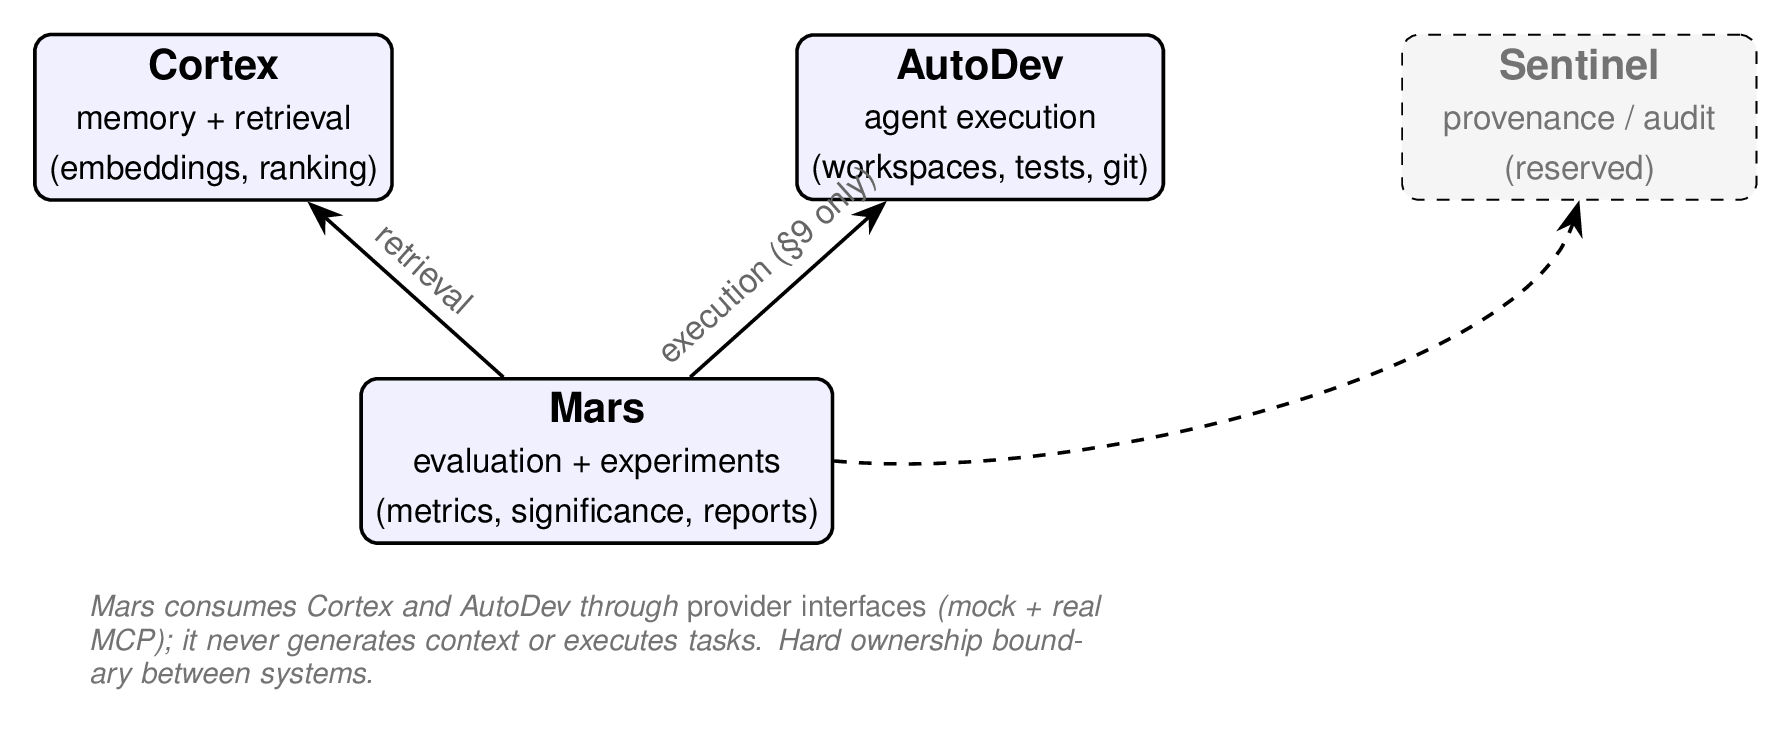
\includegraphics[width=0.92\textwidth]{figure1_architecture.png}
\caption{System architecture and the Cortex / Mars / AutoDev ownership boundary. Mars
never generates context or executes tasks; it measures.}
\label{fig:architecture}
\end{figure}

\begin{figure}[h]
\centering
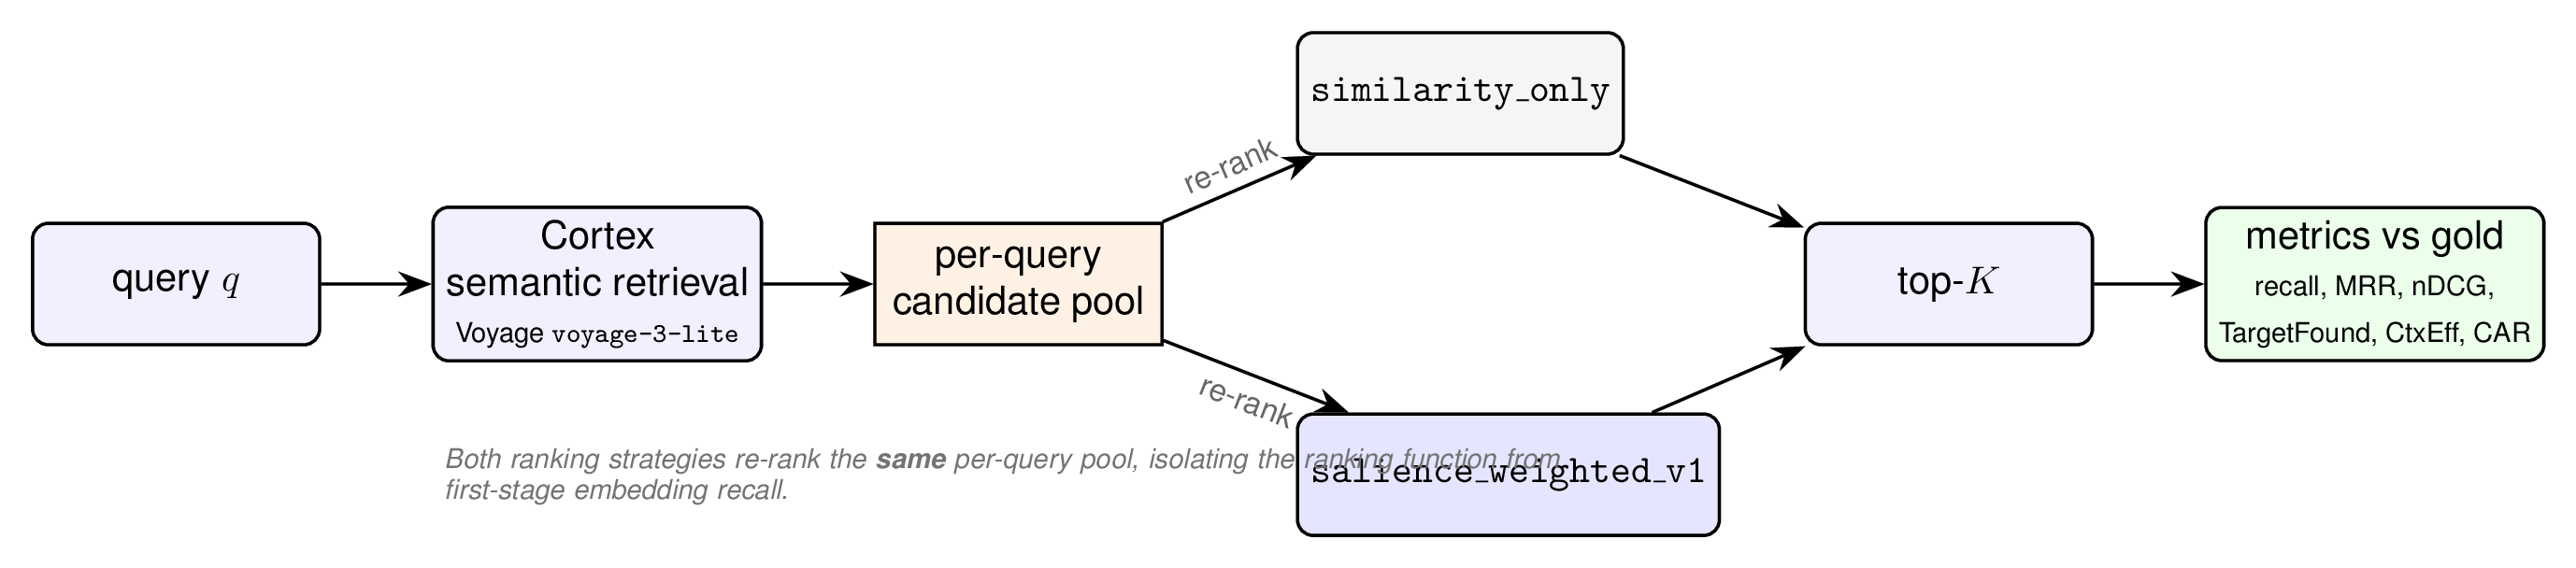
\includegraphics[width=0.92\textwidth]{figure2_pipeline.png}
\caption{The retrieval pipeline: both ranking strategies re-rank the same candidate pool,
isolating the ranking function from first-stage embedding recall.}
\label{fig:pipeline}
\end{figure}

% ===========================================================================
\section{Experimental Framework}
\label{sec:framework}
% ===========================================================================

\subsection{Infrastructure}
The evaluation uses systems with a hard ownership boundary (\cref{fig:architecture}).
\textbf{Cortex} owns memory and retrieval: storage, embeddings, semantic retrieval,
salience metadata, and ranking explanations; it serves the real semantic baseline via
Voyage \texttt{voyage-3-lite} embeddings (confirmed live, HTTP 200 per memory).
\textbf{Mars} owns experimentation: it executes the benchmark, applies ranking strategies,
computes metrics, runs significance tests, and produces reports; it does not generate
context or execute tasks. \textbf{AutoDev} owns agent execution and is exercised only in
\cref{sec:exp5}. \textbf{Sentinel} provides auditability/provenance and is a reserved
extension point.

An honesty constraint is enforced in the framework: if the backend cannot supply semantic
scores (embeddings disabled $\to$ \texttt{semantic\_score: null}), the run is flagged and
the report is forbidden from claiming a semantic-vs-salience result. All retrieval results
below were produced with \texttt{semantic\_score} verified non-null.

\subsection{Benchmark corpus}
Salience Memory Benchmark v1 is a synthetic, labeled retrieval benchmark of 30 queries and
552 memories ($\sim$18/query) across six categories (\cref{fig:corpus,tab:corpus}). Each
query has exactly one \emph{target} memory, a set of \emph{relevant} support memories, and
a controlled pool of adversarial memories. Gold relevance is explicit per query, so ranking
and coverage are both measurable.

\begin{table}[h]
\centering
\caption{Salience Memory Benchmark v1 corpus composition.}
\label{tab:corpus}
\begin{tabular}{lrl}
\toprule
Category & Count & Role \\
\midrule
\texttt{target} & 30 & One primary memory per query (gold target). \\
\texttt{relevant} & 102 & Helpful support memories. \\
\texttt{distractor} & 210 & High overlap, low utility; engineered to mislead similarity. \\
\texttt{stale} & 90 & Previously useful, now outdated. \\
\texttt{contradictory} & 30 & Conflict with the truth. \\
\texttt{low\_confidence} & 90 & Possibly incorrect (low authored confidence). \\
\midrule
\textbf{Total} & \textbf{552} & 30 queries. \\
\bottomrule
\end{tabular}
\end{table}

The corpus is \textbf{adversarial by construction}: distractors are written to be
\emph{semantically closer} to the query than the truly relevant memories while carrying low
importance. This is the long-horizon failure mode the study targets, and it is what makes
the benchmark discriminating --- an earlier 13-memory smoke test saturated at recall@5
$=1.0$ for every strategy. The corpus is authored reproducibly by a committed generator and
is frozen and hash-pinned (v1.0.0, SHA256 \texttt{a464085c\ldots}); bytes are never
silently mutated, and \texttt{mars corpus verify-frozen} plus a CI check guard the
invariant.

\begin{figure}[h]
\centering
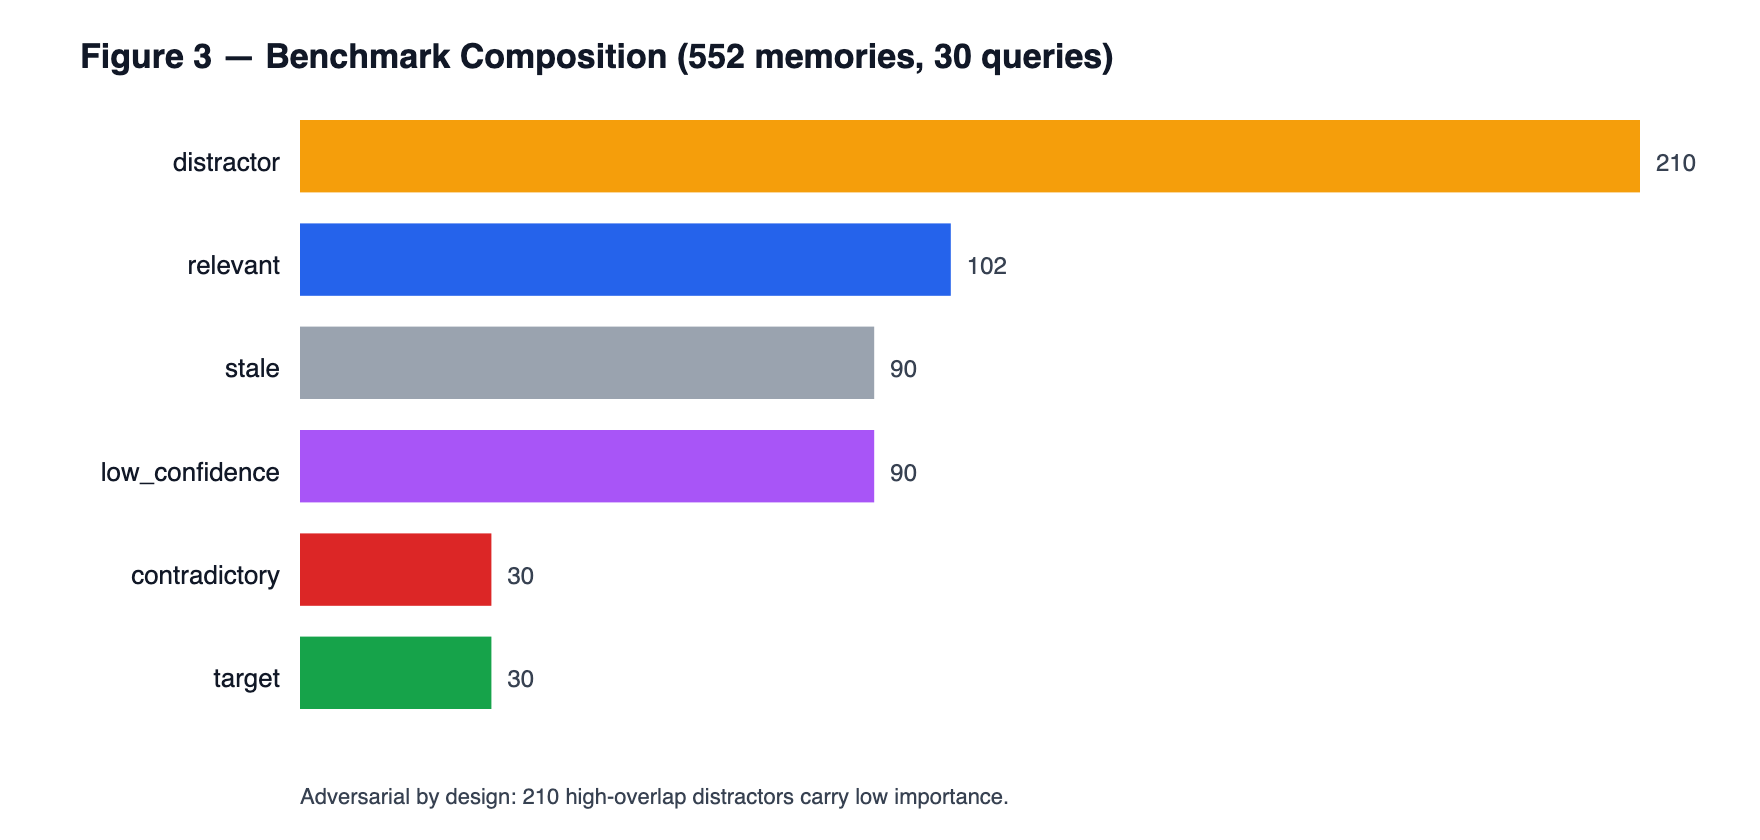
\includegraphics[width=0.8\textwidth]{figure3_corpus_composition.png}
\caption{Benchmark composition: 210 high-overlap distractors dominate the corpus, so a
ranker must use something beyond similarity to win.}
\label{fig:corpus}
\end{figure}

\subsection{Metrics}
For gold set $G(q)$ and ranked output, averaged over the 30 queries: \textbf{Recall@K} /
\textbf{Precision@K} (coverage of $G(q)$ in the top $K$), \textbf{MRR} (mean reciprocal
rank of the target), \textbf{nDCG@K} (graded ranking quality), \textbf{TargetFound@K}
(fraction of queries whose single target appears in the top $K$), and
\textbf{ContextEfficiency@K} (fraction of the top-$K$ budget spent on gold-relevant
memories). Experiment 4 adds \textbf{ContradictionAvoidanceRate (\car)}: over
contradiction-eligible queries (28/30), the fraction where the correct target outranks
\emph{every} obsolete contradictory memory. Full definitions appear in
\cref{app:metrics}.

\subsection{Statistical testing}
Significance is a \textbf{paired bootstrap}~\cite{efron1986bootstrap} (10{,}000 resamples)
over the 30-query distribution: we resample queries with replacement, recompute
per-strategy means, and report the 95\% CI of the difference (salience $-$ baseline).
Because both strategies re-rank the same pool per query, the comparison is naturally
paired; we also report per-query win/tie/loss tallies. Retrieval is deterministic given
fixed embeddings, so the reported uncertainty is over the query distribution, not
run-to-run noise. Experiments 2--4 reuse a committed real-retrieval cache so their sweeps
are offline and deterministic; Experiment 2 uses 25 seeds/level.

% ===========================================================================
\section{Experiment 1 --- Salience Retrieval}
\label{sec:exp1}
% ===========================================================================

\paragraph{Question.} Does salience-weighted retrieval beat semantic-similarity-only
retrieval?

\paragraph{Setup.} Real Cortex retrieval over MCP with Voyage \texttt{voyage-3-lite}
embeddings; mock execution (retrieval-only). Baseline \texttt{similarity\_only}; candidate
\texttt{salience\_weighted\_v1} with weights $(0.40, 0.30, 0.20, 0.10)$.

\paragraph{Results} (\cref{tab:exp1}, \cref{fig:exp1}).

\begin{table}[h]
\centering
\caption{Experiment 1: salience-weighted vs.\ similarity-only retrieval.}
\label{tab:exp1}
\begin{tabular}{lrrr}
\toprule
Metric & \texttt{similarity\_only} & \texttt{salience\_weighted\_v1} & $\Delta$ \\
\midrule
recall@1 & 0.067 & 0.933 & $+0.867$ \\
recall@5 & 0.237 & 0.672 & $\mathbf{+0.435}$ \\
recall@10 & 0.761 & 0.931 & $+0.169$ \\
MRR & 0.313 & 0.967 & $\mathbf{+0.654}$ \\
nDCG@5 & 0.184 & 0.714 & $\mathbf{+0.531}$ \\
TargetFound@3 & 0.367 & 1.000 & $+0.633$ \\
TargetFound@5 & 0.667 & 1.000 & $+0.333$ \\
ContextEfficiency@5 & 0.200 & 0.567 & $+0.367$ \\
\bottomrule
\end{tabular}
\end{table}

Paired significance: recall@5 $+0.435$ (95\% CI $[+0.367, +0.502]$, 29/1/0 win/tie/loss);
nDCG@5 $+0.531$ (95\% CI $[+0.474, +0.583]$, 30/0/0). Both intervals exclude zero by a wide
margin; every metric improves. MRR $0.31\to0.97$ means the right memory went from ``usually
buried'' to ``almost always ranked first.''

\begin{figure}[h]
\centering
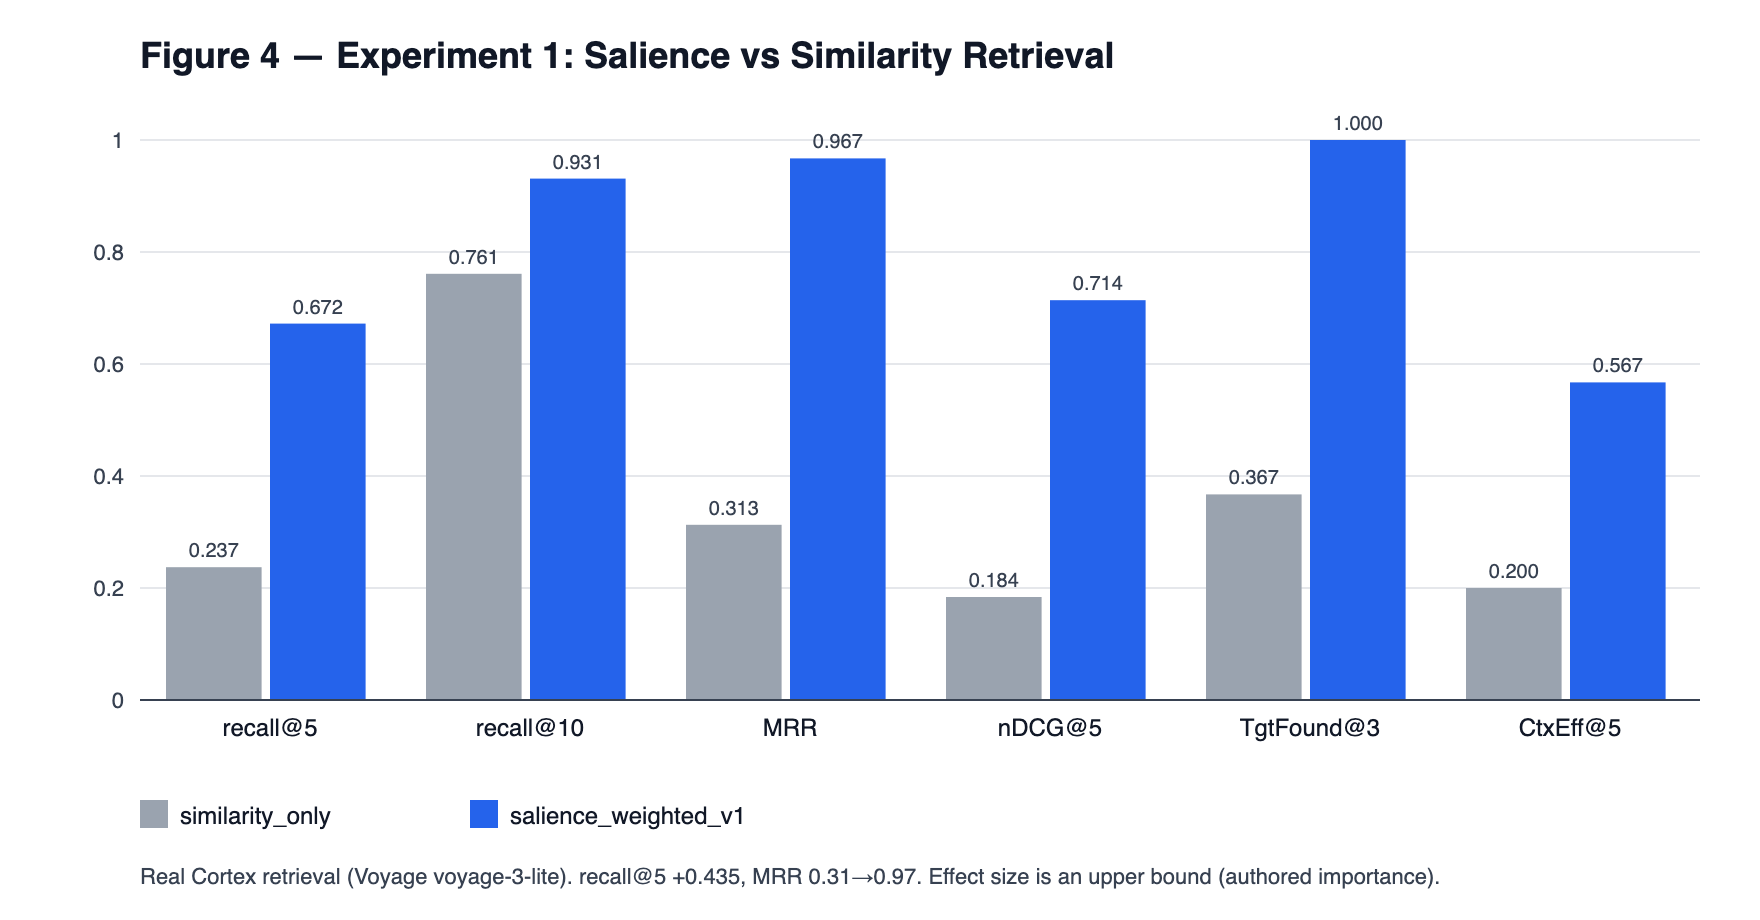
\includegraphics[width=0.9\textwidth]{figure4_exp1_results.png}
\caption{Experiment 1: importance-weighted vs.\ similarity-only across the metric suite.}
\label{fig:exp1}
\end{figure}

\paragraph{Mechanism (verified live)} (\cref{fig:ranking}). On the migration query, the
top semantic matches are three distractors ($\mathrm{sim}\approx0.77$--$0.79$,
$\mathrm{importance}\approx0.04$--$0.07$) and a contradictory memory, burying the target at
rank 6. The importance term (relevant $\gg$ distractor by construction) lifts the relevant
memories above the distractors, moving the target to rank 1. This is the corpus's designed
mechanism operating as intended, not a metric artifact.

\begin{figure}[h]
\centering
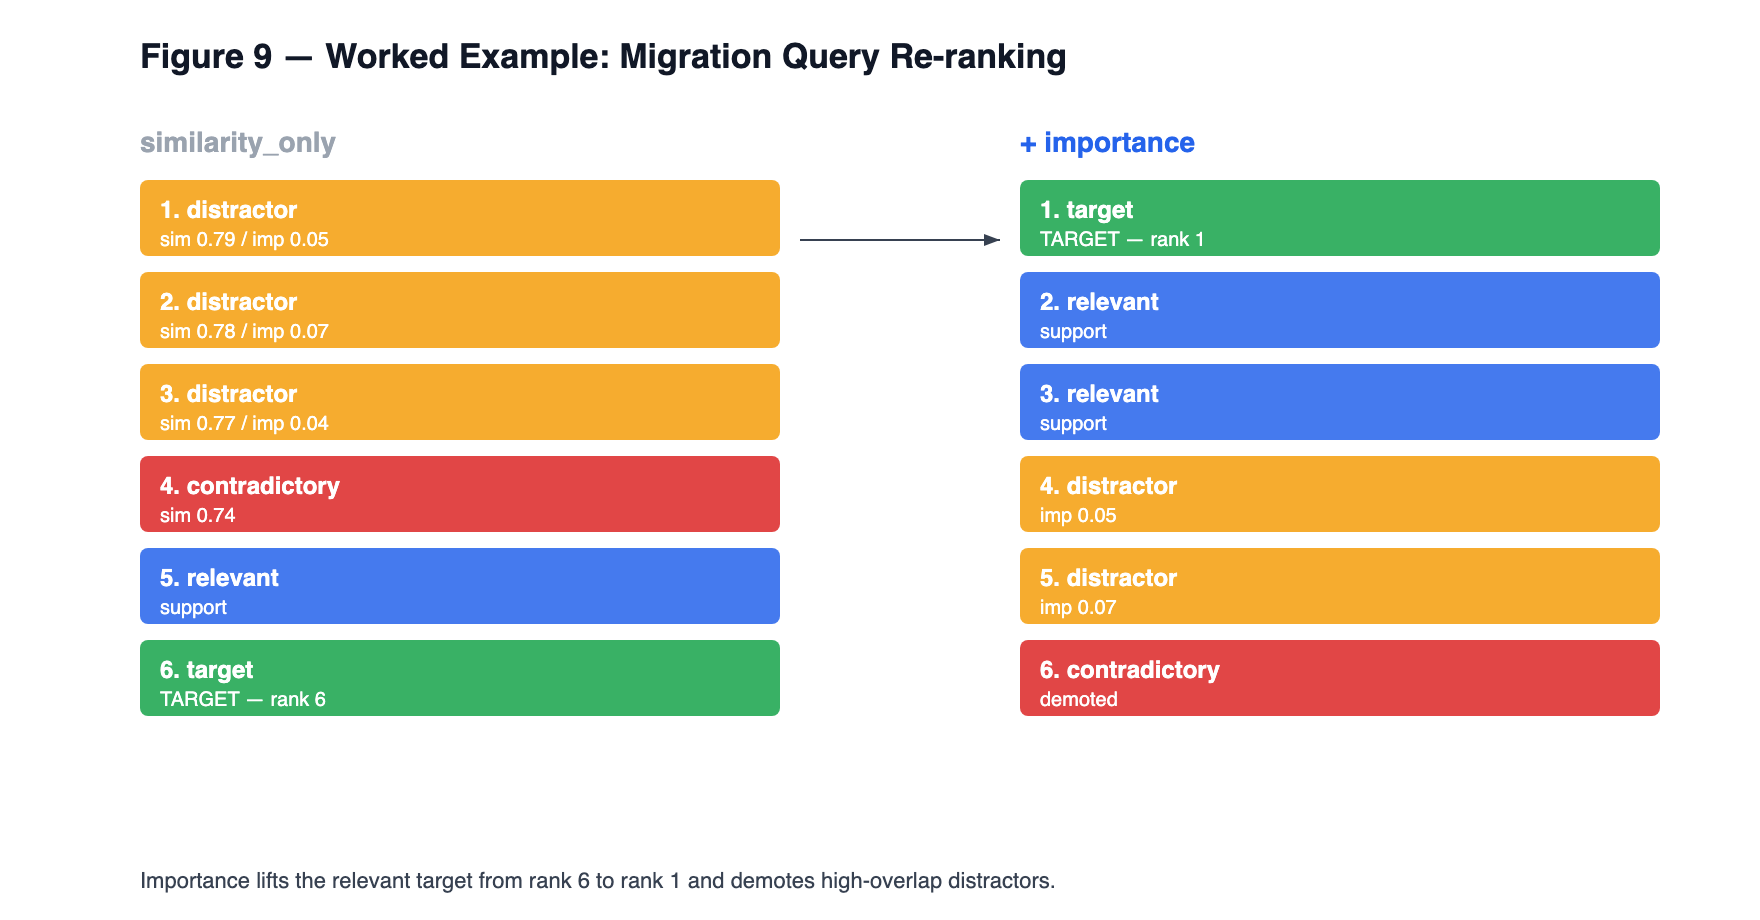
\includegraphics[width=0.85\textwidth]{figure9_ranking_example.png}
\caption{A worked example: adding importance moves the target memory from rank 6 to rank 1
on the database-migration query.}
\label{fig:ranking}
\end{figure}

\paragraph{Finding.} Salience-weighted retrieval clearly and significantly improves both
ranking and coverage on a non-saturating benchmark with a real semantic baseline. The
effect size is an \textbf{upper bound}: importance is an authored oracle here (relevant
high, distractors low). Recency and frequency contribute nothing (all memories seeded at
once) --- the entire win is importance-driven, which \cref{sec:exp2} then stress-tests.

% ===========================================================================
\section{Experiment 2 --- Noisy Importance}
\label{sec:exp2}
% ===========================================================================

\paragraph{Question.} How much of the win survives when importance is noisy rather than a
clean oracle? (This section exists to answer the circularity objection to \cref{sec:exp1}:
\emph{you just encoded the answer into the labels.})

\paragraph{Setup.} Same corpus and real retrieval, with importance degraded by a shuffle
model (a fraction $1-\mathrm{quality}$ of each pool's importance values permuted among
themselves) across a quality grid $1.00\to0.00$, 25 seeds/level. Importance is corrupted
\emph{post-retrieval} (it never affects the embeddings or the retrieved pool), faithful to
re-seeding Cortex with corrupted labels. The oracle level reproduces Experiment 1 exactly,
validating the pipeline.

\paragraph{Results} (\cref{tab:exp2}, \cref{fig:exp2}).

\begin{table}[h]
\centering
\caption{Experiment 2: recall@5 as importance quality is degraded toward random.}
\label{tab:exp2}
\begin{tabular}{lrlr}
\toprule
importance quality & recall@5 & $\Delta$ recall@5 (95\% CI) & MRR \\
\midrule
1.00 (oracle) & 0.672 & $+0.435$ $[+0.370, +0.503]$ & 0.967 \\
0.75 & 0.593 & $+0.356$ $[+0.302, +0.414]$ & 0.864 \\
0.50 & 0.506 & $+0.269$ $[+0.218, +0.322]$ & 0.746 \\
0.25 & 0.420 & $+0.183$ $[+0.142, +0.224]$ & 0.584 \\
0.00 (scrambled) & 0.330 & $+0.094$ $[+0.050, +0.139]$ & 0.423 \\
\bottomrule
\end{tabular}
\end{table}

\begin{figure}[h]
\centering
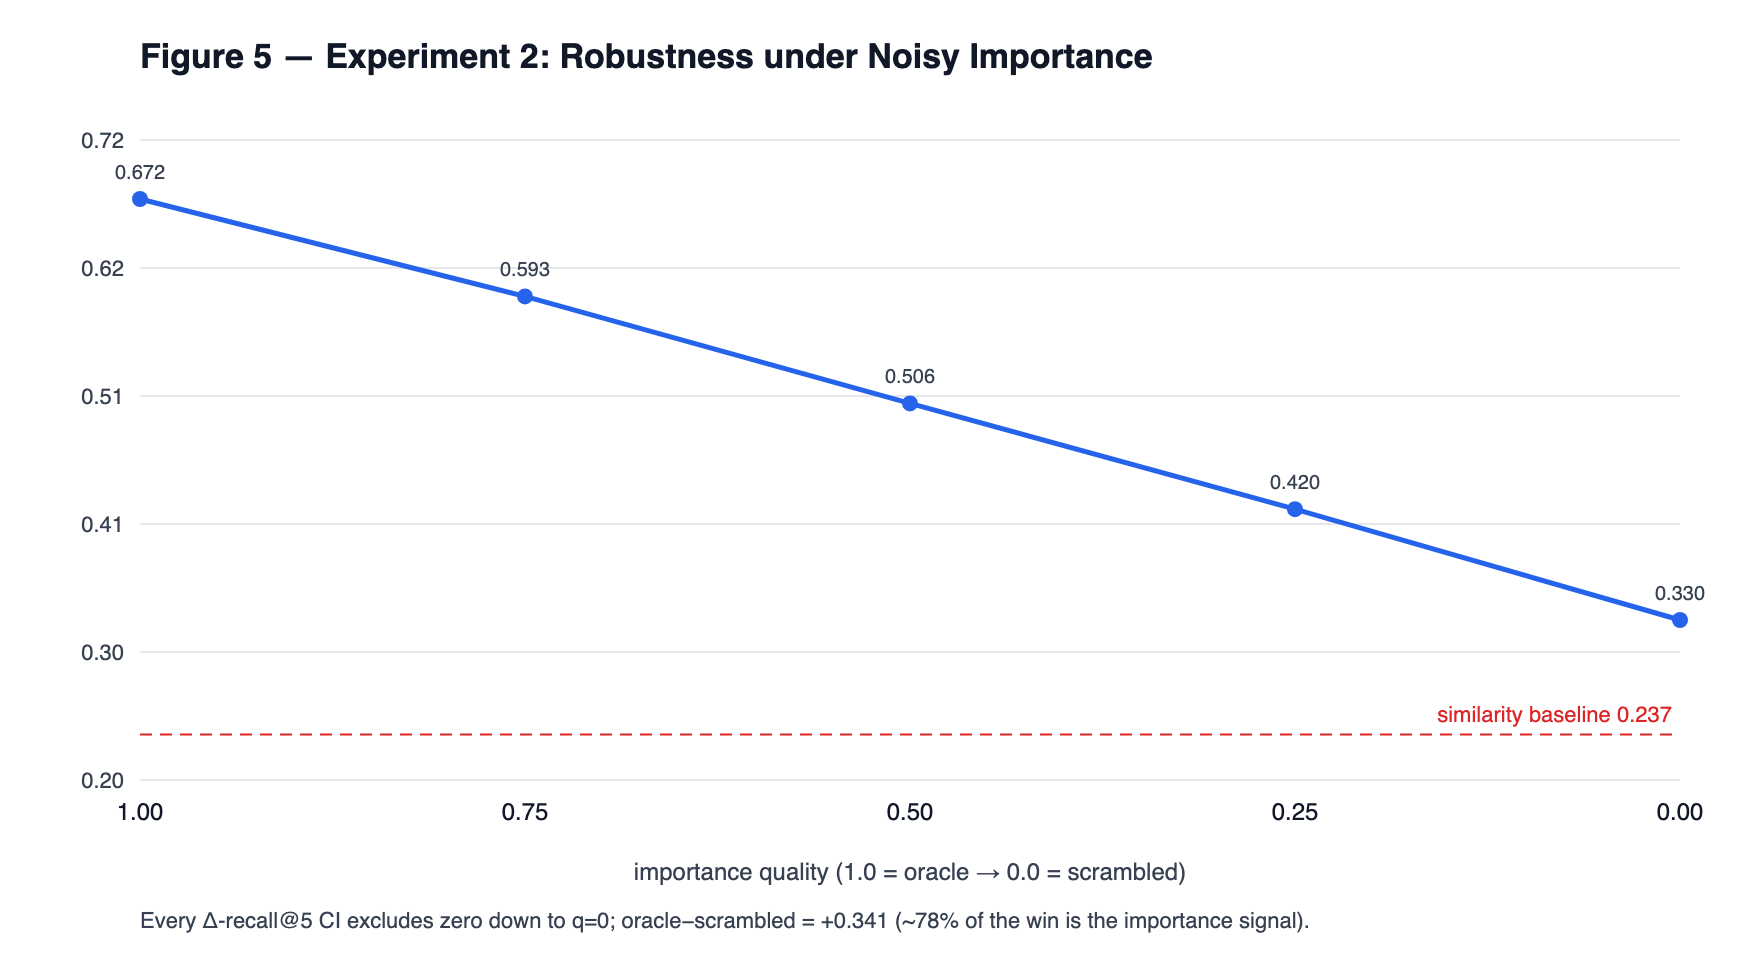
\includegraphics[width=0.85\textwidth]{figure5_noisy_importance.png}
\caption{Noisy importance: the advantage decays smoothly and monotonically and never
reaches the similarity baseline.}
\label{fig:exp2}
\end{figure}

\paragraph{Finding.} Degradation is \textbf{graceful and monotonic} --- there is no cliff,
and every CI excludes zero, so the salience arm beats plain semantic retrieval at every
tested importance quality. The honest measure of the importance \emph{signal's}
contribution is oracle $-$ scrambled (recall@5 $0.672\to0.330 = +0.341$), i.e.\
$\sim$78\% of the advantage is carried by the importance signal itself. The residual
$+0.094$ at $q=0$ is not information: when we instead zero out the importance term entirely,
recall collapses exactly back to the similarity baseline ($0.237$). The residual is the
stochastic perturbation of random importance values breaking ties in this corpus's
adversarial similarity ordering --- a perturbation effect, not a signal.

\paragraph{Decision.} Salience weighting is robust to substantial importance noise; it does
not need a near-perfect importance estimate to pay off. This bounds, but does not eliminate,
the \cref{sec:exp1} ceiling caveat: the effect is not purely an artifact of clean labels.

% ===========================================================================
\section{Experiment 3 --- Temporal Salience}
\label{sec:exp3}
% ===========================================================================

\paragraph{Question.} Does recency improve or degrade salience-weighted retrieval, and does
it earn a place as a core signal?

\paragraph{Setup.} Reuses the committed real-retrieval cache (nothing re-embedded); only
synthetic timestamps and strategy vary. Four regimes: \textbf{A uniform} (control),
\textbf{B recency-aligned} (relevant newer), \textbf{C recency-misaligned} (distractors
newer), \textbf{D mixed-realistic} (ages independent of relevance). The recency
\emph{marginal} is isolated as
$\texttt{importance\_plus\_recency} - \texttt{sim\_plus\_importance}$ (identical
similarity/importance weights; the delta is the $0.10$ recency term alone).

\paragraph{Results --- isolated recency marginal} (recall@5, paired 95\% CI;
\cref{tab:exp3}, \cref{fig:exp3}).

\begin{table}[h]
\centering
\caption{Experiment 3: isolated recency marginal across four timestamp regimes.}
\label{tab:exp3}
\begin{tabular}{lll}
\toprule
Regime & marginal & verdict \\
\midrule
A uniform & $+0.000$ $[+0.000, +0.000]$ & neutral (control passes) \\
B aligned & $+0.262$ $[+0.210, +0.316]$ & recency \textbf{helps} \\
C misaligned & $-0.206$ $[-0.262, -0.155]$ & recency \textbf{hurts} \\
D mixed realistic & $+0.015$ $[-0.025, +0.055]$ & \textbf{neutral} (CI spans 0) \\
\bottomrule
\end{tabular}
\end{table}

\texttt{importance\_only} is \textbf{regime-invariant} at recall@5 $0.985$ / MRR $1.000$
across all four regimes --- time neither helps nor harms importance.

\begin{figure}[h]
\centering
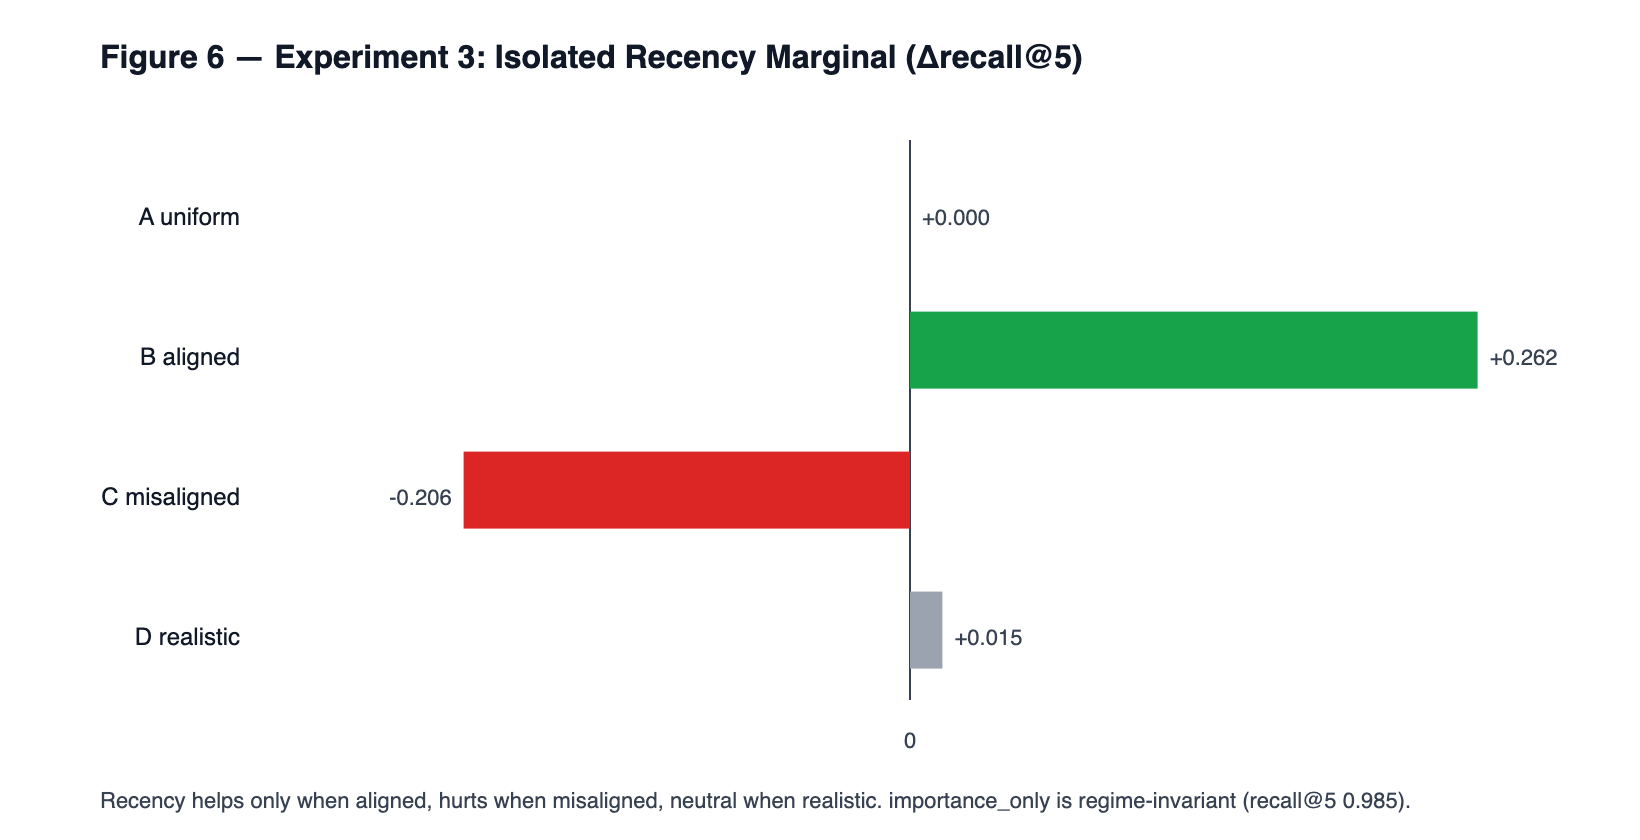
\includegraphics[width=0.85\textwidth]{figure6_temporal_salience.png}
\caption{Temporal salience: recency's effect flips sign depending on the regime, while
importance is flat across all four.}
\label{fig:exp3}
\end{figure}

\paragraph{Finding.} Raw recency helps only in the artificial aligned regime, hurts by a
nearly symmetric amount when misaligned, and is statistically neutral in the realistic
mixed regime. Importance dominates everywhere. The safest temporal strategy is a
short-half-life decay ($\approx$7 days) --- the only temporal arm that significantly beats
the similarity baseline in \emph{every} regime --- but it never beats
\texttt{importance\_only}.

\paragraph{Decision.} Recency is \textbf{not promoted} to a core signal. At best it is an
optional short-decay, low-weight, importance-gated add-on. Reporting this negative result as
a design decision is itself a contribution: a plausible signal that fails its ablation is
removed.

% ===========================================================================
\section{Experiment 4 --- Confidence \& Contradiction}
\label{sec:exp4}
% ===========================================================================

\paragraph{Question.} Can confidence-aware retrieval help agents avoid outdated, incorrect,
or contradictory memories --- especially when an important memory is wrong?

\paragraph{Setup.} Reuses the cached pools joined to the corpus by content to recover each
memory's authored \texttt{category} and \texttt{confidence}. Five confidence regimes,
including an adversarial \textbf{E ``important-but-wrong''} regime where the obsolete memory
is forced to be \emph{slightly more important than the target} but low-confidence. New
metric: ContradictionAvoidanceRate (\car) over the 28/30 contradiction-eligible queries.
Compares additive confidence
($0.65\,\mathrm{sim} + 0.25\,\mathrm{imp} + 0.10\,\mathrm{conf}$) vs.\ \textbf{gated}
confidence ($0.65\,\mathrm{sim} + 0.35\,(\mathrm{imp}\times\mathrm{conf})$).

\paragraph{Results --- ContradictionAvoidanceRate} (\cref{tab:exp4}, \cref{fig:exp4}).

\begin{table}[h]
\centering
\caption{Experiment 4: ContradictionAvoidanceRate across five confidence regimes.}
\label{tab:exp4}
\begin{tabular}{lrrrrr}
\toprule
Strategy & A & B & C & D & E (imp.-but-wrong) \\
\midrule
\texttt{similarity\_only} & 0.643 & 0.643 & 0.643 & 0.643 & 0.643 \\
\texttt{importance\_only} & 1.000 & 1.000 & 1.000 & 1.000 & \textbf{0.000} \\
\texttt{confidence\_only} & 0.479 & 1.000 & 1.000 & 1.000 & 1.000 \\
$\mathrm{imp}\times\mathrm{conf}$ (gated) & 0.964 & 0.964 & 0.964 & 0.964 & \textbf{0.964} \\
\bottomrule
\end{tabular}
\end{table}

The isolated confidence marginal (recall@5) is positive and significant wherever confidence
is informative (B $+0.265$, C $+0.169$, D $+0.108$, E $+0.146$) and $\approx0$ in the
control (A $+0.010$).

\begin{figure}[h]
\centering
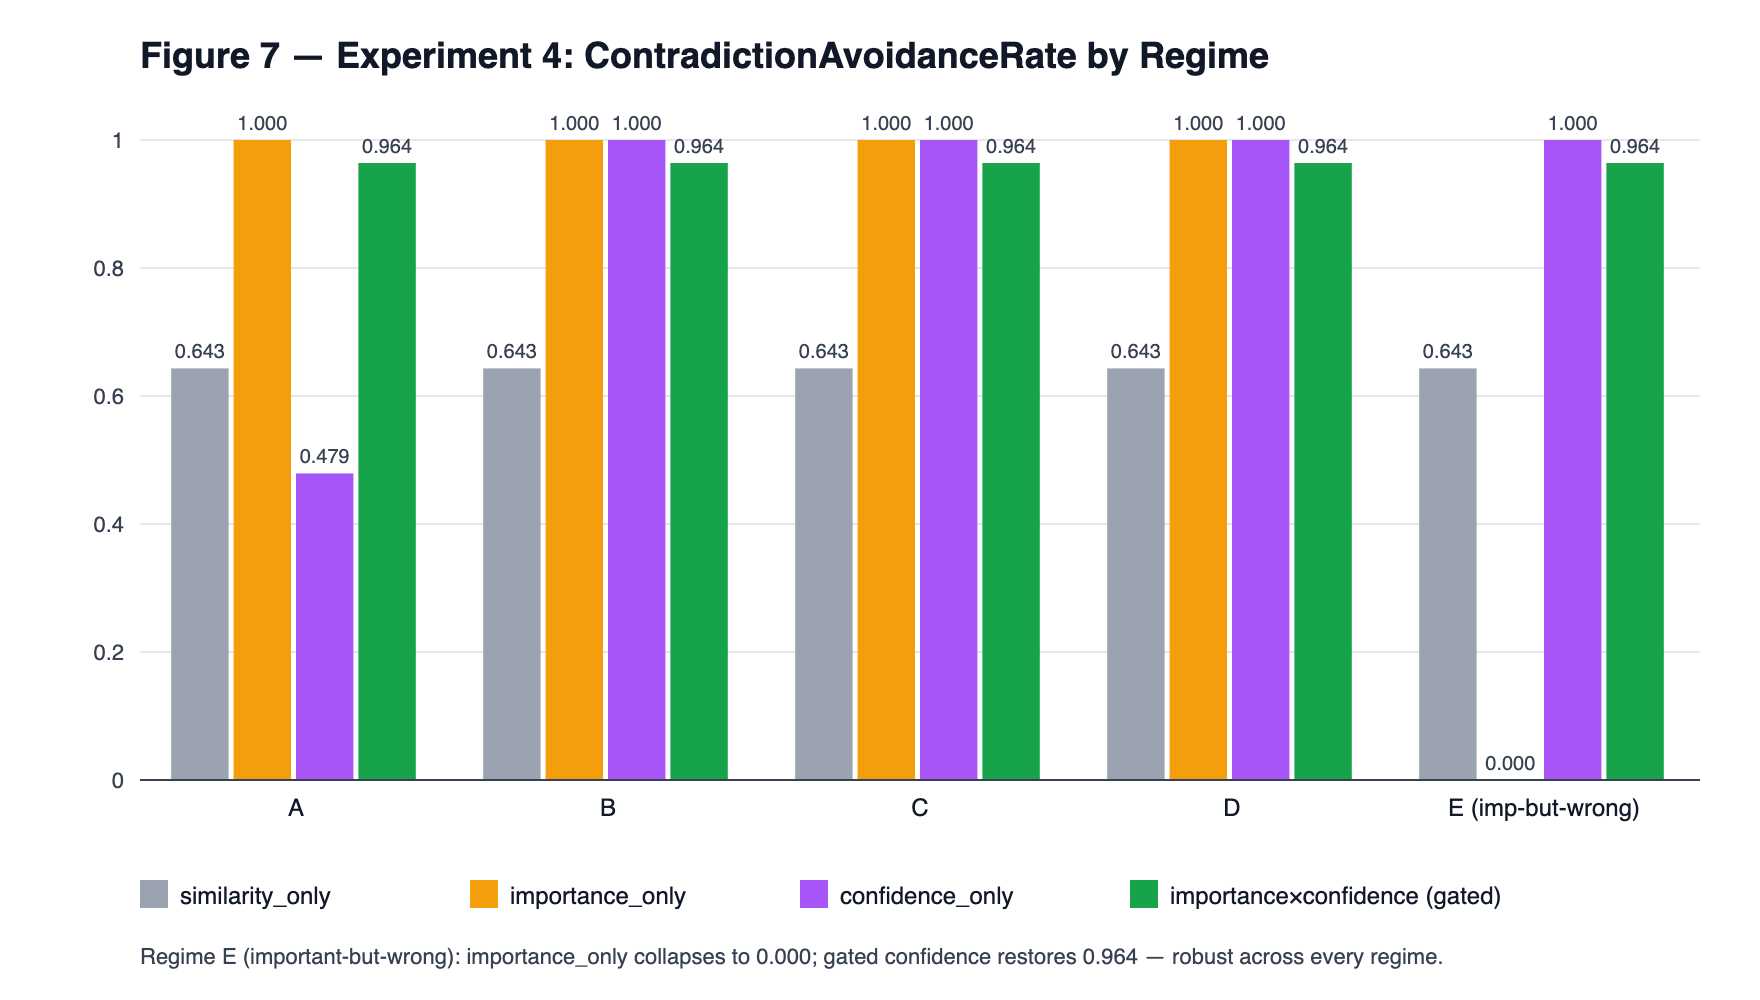
\includegraphics[width=0.85\textwidth]{figure7_confidence_contradiction.png}
\caption{Confidence and contradiction: only the gated form is robust across every regime,
including the adversarial important-but-wrong regime E.}
\label{fig:exp4}
\end{figure}

\paragraph{Finding.} In the easy regimes (A--D), importance already achieves perfect
avoidance, so confidence is redundant. In the adversarial regime E, \texttt{importance\_only}
collapses to \textbf{\car{} $0.000$} (it ranks the important-but-wrong memory first in all 28
queries) --- and \textbf{confidence-gating restores avoidance to $0.964$}, the only
importance-based strategy robust across \emph{every} regime. Confidence's unique,
non-redundant value appears exactly when importance and confidence diverge.

\paragraph{Decision.} Confidence \textbf{joins importance as a core signal, in gated
(multiplicative) form} ($\mathrm{eff\_imp} = \mathrm{imp}\times\mathrm{conf}$). It is
redundant-but-harmless when the two agree and decisive when they diverge. Recency stays out.
The \emph{form} of the signal matters: the multiplicative gate produces robustness; an
additive term does not.

% ===========================================================================
\section{Experiments 5 \& 5.1 --- Execution Impact}
\label{sec:exp5}
% ===========================================================================

\subsection{Experiment 5 (methodology milestone)}
We wired Mars to drive a real AutoDev agent over MCP across all three retrieval arms (A
\texttt{similarity\_only}, B \texttt{sim\_importance}, C \texttt{salience\_v2}), injecting
per-arm context via \texttt{start\_run(retrieval\_strategy=$\ldots$, context\_package\_id=$\ldots$)}.
A divergence gate confirmed the arms inject \textbf{different} contexts
(\texttt{arms\_distinct=true}, \texttt{valid\_comparison=true}). Retrieval improved as
predicted inside the real pipeline (recall@5 $0.50\to0.83$, MRR $0.28\to0.57$, target-found
$0.50\to1.00$, \car{} $0.00\to1.00$ over 18 runs, $\approx\$1.55$). However,
\textbf{task-success floored at $0.000$ for all three arms} (the dry-run coder solved no
task regardless of context). With zero success variance, the retrieval$\leftrightarrow$success
correlation was trivially $0.000$ and \emph{uninformative} --- not evidence of ``no
relationship.'' Experiment 5 thus established the pipeline but could not answer the
execution-impact question, motivating a purpose-built, less-floored benchmark.

\subsection{Experiment 5.1 (first evidential result)}
\paragraph{Setup.} A purpose-built, memory-dependent benchmark: six tasks in a small,
dependency-free repo, each requiring knowledge that lives in a decision/postmortem/convention
not visible in the edited file --- or actively contradicted by a stale doc still present in
the repo. Each task gets an isolated 5-record store, reseeded before every run: one
\textbf{corrective} record (importance 3.5, old, deliberately low term-overlap) plus four
recent, higher-overlap distractors. A pure-similarity ranker buries the corrective record;
importance-aware rankers surface it. 18 real AutoDev runs (6 tasks $\times$ 3 arms $\times$
1 trial), dry-run, \texttt{retrieval\_limit=3}, $\approx\$1.3$. Success oracle $=$ the
task's targeted test with the test file forbidden; Mars restores forbidden files before
validating, so success reflects the agent's implementation against a fixed oracle.

\paragraph{Results} (\cref{tab:exp5}, \cref{fig:exp5}).

\begin{table}[h]
\centering
\caption{Experiment 5.1: 18 real AutoDev runs across three retrieval arms.}
\label{tab:exp5}
\begin{tabular}{lrrrrr}
\toprule
Arm & Task success & recall@5 & Target found & MRR & Right-approach \\
\midrule
A --- \texttt{similarity\_only} & 0.333 & 0.000 & 0.000 & 0.000 & 0.833 \\
B --- \texttt{sim+importance} & 0.333 & 0.833 & 0.833 & 0.556 & 1.000 \\
C --- \texttt{salience\_v2} & 0.333 & 0.833 & 0.833 & 0.556 & 1.000 \\
\bottomrule
\end{tabular}
\end{table}

Paired $\Delta$ success vs.\ A: B $+0.000$ (6 ties), C $+0.000$ (6 ties). At
\texttt{limit=3} the similarity arm \textbf{never} injects the corrective record
(recall/target-found $0.0$), while both importance arms inject it $\sim$5/6 of the time; B
and C are identical because the recency term in \texttt{salience\_v2} reorders but does not
change the top-3 set (consistent with \cref{sec:exp3}).

\begin{figure}[h]
\centering
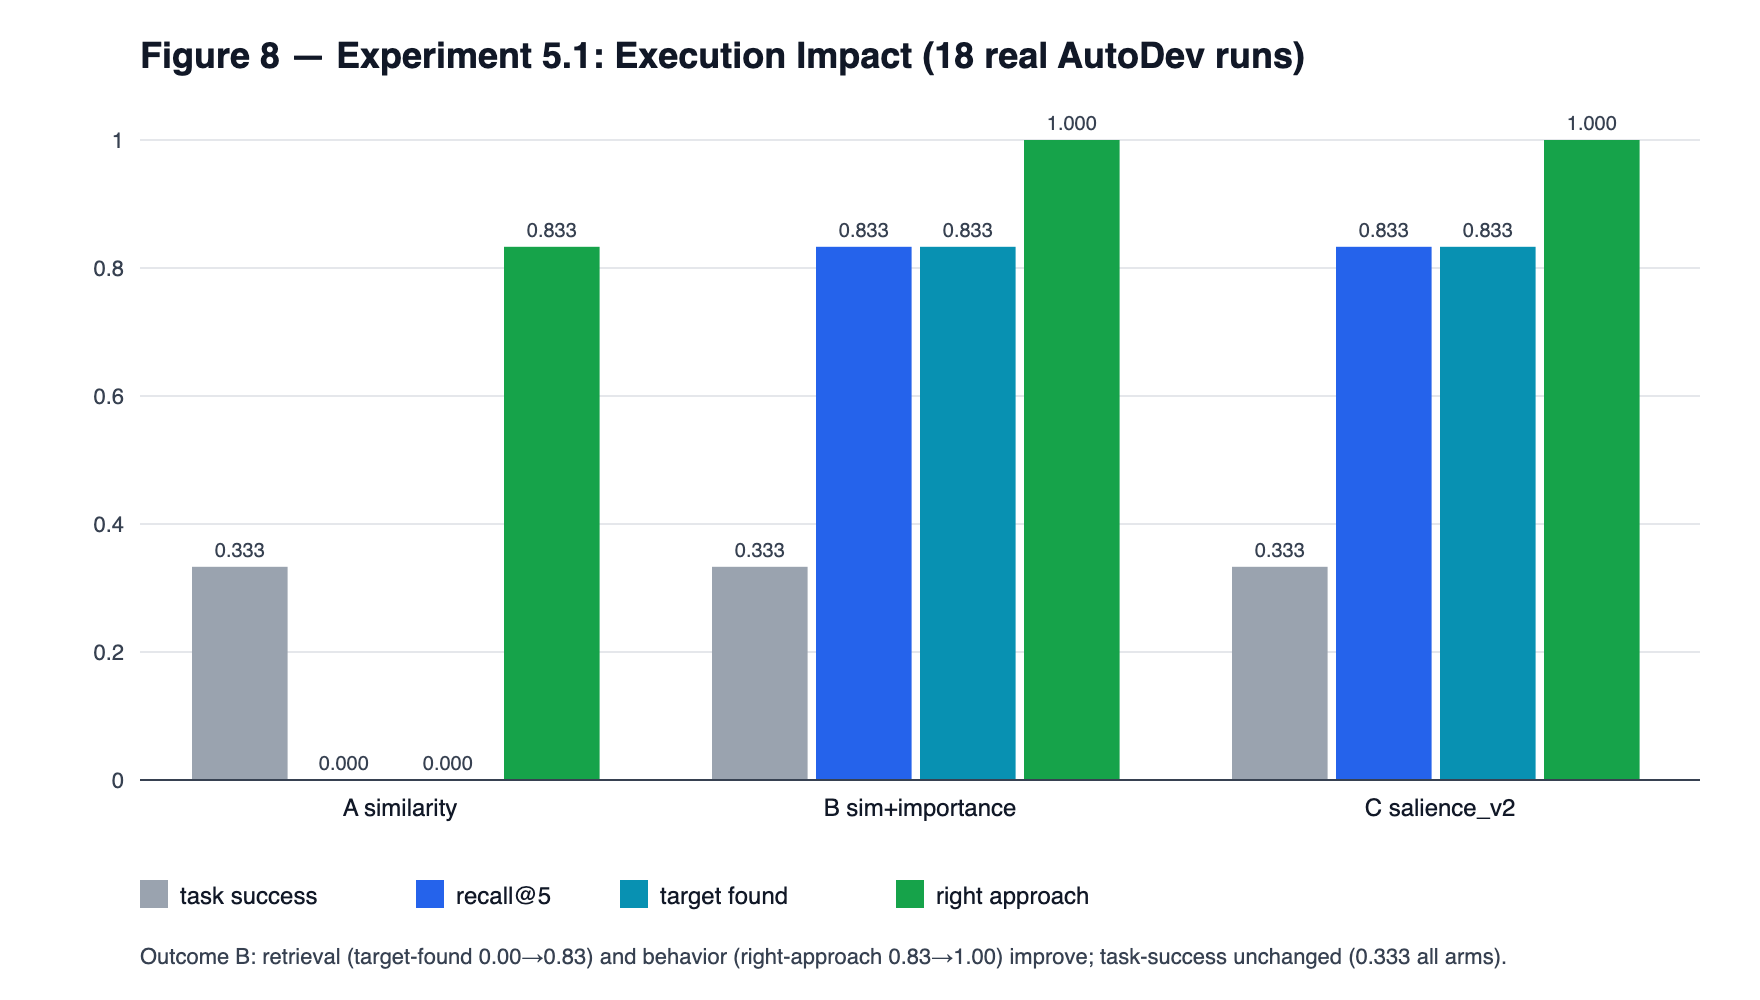
\includegraphics[width=0.9\textwidth]{figure8_execution_impact.png}
\caption{Execution impact: retrieval quality and ``right approach'' rise across the
importance arms while task-success stays flat at $0.333$.}
\label{fig:exp5}
\end{figure}

\paragraph{Behavioral analysis.} The clearest case is \texttt{bench-4}
(protect-admin-reports), whose \texttt{docs/AUTH.md} is stale. Arm A, deprived of the
corrective memory, trusted the out-of-date doc and implemented \textbf{session-cookie}
auth; arms B/C, given the corrective memory, implemented the repo's current \textbf{JWT}
convention. Across the suite, the right-approach rate is \textbf{$1.00$ for B/C vs.\ $0.83$
for A} --- a genuine, observed retrieval$\to$behavior effect. It was simply not enough to
pass the stricter, multi-assertion oracle within the iteration budget. The contradiction
finding from \cref{sec:exp4} also replicated at the agent layer: the similarity arm's
dominant failure mode is retrieving a contradiction and acting on it (4/6 tasks), versus
1/6 for each importance arm.

\paragraph{Outcome.} \textbf{Outcome B: retrieval improves, behavior changes, task-success
does not.} The recall$\leftrightarrow$success correlation is slightly \textbf{negative}
(Pearson $-0.32$), an artifact of \emph{which} tasks are winnable: the 2 passing tasks are
discoverable-from-code (the similarity arm passes them with recall $0$), while the tasks
where retrieval helped most (the contradiction tasks) are also the hardest to implement and
fail anyway. Downstream pass/fail here is dominated by implementation quality and a per-task
difficulty floor (4/6 tasks fail in every arm at \texttt{max\_iterations=3}), not by which
memories were retrieved.

We \textbf{do not} claim salience improves agent task outcomes. The supported claim is:
salience improves retrieval and steers the agent toward the repository's current
conventions; on this benchmark that did not yet raise task-success. This is the discipline
the whole study is built around: retrieval quality is a proxy, task-success is the outcome,
and the two came apart here.

% ===========================================================================
\section{Discussion}
\label{sec:discussion}
% ===========================================================================

\paragraph{Salience as prioritization.} Across the retrieval studies, a small number of
non-similarity scalars reorder a pool that similarity has mis-ordered, surfacing
consequential-but-unremarkable memories and demoting high-overlap distractors. In the
language of attention allocation, the agent spends more of its limited context budget on
memories that matter. We make no cognitive or affective claim beyond this.

\paragraph{Supported vs.\ unsupported claims.} We keep these strictly separate.

\emph{Supported:} salience improves retrieval quality (\cref{sec:exp1}); the gain is robust
to importance noise (\cref{sec:exp2}); recency is weak and not promoted (\cref{sec:exp3});
confidence, as a gate, prevents contradiction failures (\cref{sec:exp4}); improved retrieval
changes agent behavior (\cref{sec:exp5}).

\emph{Unsupported:} salience improves agent task-success; salience improves production
outcomes; salience generalizes beyond the tested corpus, weight set, and embedding model.

\paragraph{Threats to validity.} The most serious is \emph{construct circularity}:
importance and relevance are correlated by authoring, so \cref{sec:exp1}'s effect is an
upper bound --- \cref{sec:exp2} bounds but does not eliminate this. The corpus is synthetic;
external validity is unestablished. Execution is underpowered (a floor in
\cref{sec:exp5}.1's predecessor; single trial, 6 tasks, dry-run), so the execution study has
little power to detect a task-success gain even if one existed --- this is the central caveat
on every execution sentence. Absolute blend numbers are corpus-specific: one weight set, one
embedding model.

% ===========================================================================
\section{Limitations}
\label{sec:limitations}
% ===========================================================================
\begin{itemize}[leftmargin=1.4em,itemsep=2pt]
\item \textbf{Synthetic benchmark} authored by hand, not sampled from production memory
traces.
\item \textbf{Authored importance} (correlated with relevance by construction) $\to$
\cref{sec:exp1}'s effect is an upper bound.
\item \textbf{Authored confidence}; the decisive \cref{sec:exp4} regime E is a synthetic
stress test.
\item \textbf{Recency/frequency inert in \cref{sec:exp1}} (simultaneous seeding); studied
directly in \cref{sec:exp3}.
\item \textbf{Execution underpowered:} Experiment 5 floored at 0\% success; Experiment 5.1
is a single trial over 6 tasks, dry-run, with \texttt{review\_passed} unusable
(forbidden-file edits) so success uses restored-oracle validation; the 5.1 contrast exists
only at \texttt{retrieval\_limit=3}.
\item \textbf{Single embedding model} (\texttt{voyage-3-lite}) and \textbf{single weight
set} throughout.
\end{itemize}

% ===========================================================================
\section{Conclusion}
\label{sec:conclusion}
% ===========================================================================

We asked whether authored salience signals improve memory retrieval for long-horizon agents
over similarity-only ranking. On a frozen, adversarial, synthetic benchmark with a real
semantic baseline, importance-weighted retrieval improved every retrieval metric we measured
(recall@5 $+0.435$, MRR $0.31\to0.97$), the advantage survived heavy importance noise (never
collapsing to the baseline, $\sim$78\% attributable to the importance signal), recency
failed its ablation and was rejected, and confidence applied as a multiplicative gate
rescued contradiction avoidance from $0.000$ to $0.964$ when an important memory was wrong.
Inside a real agent pipeline over 18 runs, salience-aware retrieval improved retrieval and
changed the agent's behavior --- but did not raise task-success.

We keep the conclusion proportional to the evidence. Salience-weighted retrieval is a
prioritization mechanism for attention allocation over a memory store; its retrieval and
behavioral benefits are demonstrated under controlled conditions, and its effect on
downstream agent task-success remains an open, honestly-reported null. The retrieval
question is well characterized; the open frontier is execution: a larger, less-floored
execution benchmark with enough winnable tasks to give task-success statistical power;
\emph{learned} importance to replace authored labels; real-world memory traces; and
independent replication of the retrieval results.

% ===========================================================================
\section*{Reproducibility}
% ===========================================================================
The benchmark is frozen and the offline experiments require no credentials. The committed
retrieval cache makes Experiments 2--4 fully offline and deterministic; only Experiment 1
(live Voyage) and Experiment 5.1 (paid AutoDev) require credentials.
\begin{verbatim}
uv venv --python 3.12 && uv pip install -e ".[dev]"
pytest
mars corpus verify-frozen salience-memory-benchmark-v1   # integrity
python experiments/run_noisy_importance.py --cache-only  # Exp 2 (offline)
python experiments/run_temporal_salience.py              # Exp 3 (offline)
python experiments/run_confidence_contradiction.py       # Exp 4 (offline)
\end{verbatim}
Every number in this paper traces to the committed experiment artifacts
(\texttt{mars-experiments/*.json}); none are estimated for the write-up. Code, benchmark,
and figures: \url{https://github.com/alexanderjulianmartinez/mars}.

% ===========================================================================
\appendix
\section{Metric Definitions}
\label{app:metrics}
% ===========================================================================
For a query $q$ with gold set $G(q)$, ranked output, and top-$K$ prefix, averaged over the
30 queries:
\begin{itemize}[leftmargin=1.4em,itemsep=2pt]
\item \textbf{Recall@K} $= |G(q)\cap \mathrm{top}\text{-}K| / |G(q)|$.
\item \textbf{Precision@K} $= |G(q)\cap \mathrm{top}\text{-}K| / K$.
\item \textbf{MRR} $=$ mean over queries of $1/\mathrm{rank}(\mathrm{target})$.
\item \textbf{nDCG@K} $= \mathrm{DCG@K}/\mathrm{IDCG@K}$, with
$\mathrm{DCG@K} = \sum_{i=1}^{K} \mathrm{rel}_i / \log_2(i+1)$ and $\mathrm{IDCG@K}$ the DCG
of the ideal ordering.
\item \textbf{TargetFound@K} $=$ mean of $\mathbf{1}[\mathrm{target}\in \mathrm{top}\text{-}K]$.
\item \textbf{ContextEfficiency@K} $=$ fraction of the injected top-$K$ budget occupied by
gold-relevant memories.
\item \textbf{ContradictionAvoidanceRate (\car)} $=$ over the contradiction-eligible queries
(28/30), the fraction where the correct target outranks \emph{every} obsolete contradictory
memory.
\end{itemize}
Implementation: \texttt{mars/memory/metrics.py}.

\section{Bootstrap Methodology}
\label{app:bootstrap}
Significance is a paired bootstrap with 10{,}000 resamples over the 30-query distribution.
Each resample draws 30 queries with replacement, recomputes the per-strategy metric mean,
and records the difference (salience $-$ baseline); we report the $2.5/97.5$ percentiles as
the 95\% CI of the difference. Because both strategies re-rank the same per-query pool, the
comparison is paired by query; we also report per-query win/tie/loss tallies. Retrieval is
deterministic given fixed embeddings, so the reported uncertainty is over the query
distribution, not run-to-run noise. Experiment 2 additionally averages over 25 seeds per
importance-quality level; Experiments 3--4 average over seeds per regime. The paired-arm
comparison logic lives in \texttt{mars/apollo/} (\texttt{compare\_arms}).

\section{Weighting Parameters}
\label{app:weights}
\begin{itemize}[leftmargin=1.4em,itemsep=2pt]
\item \texttt{similarity\_only} (baseline): $s(q,m) = \mathrm{sim}(q,m)$.
\item \texttt{salience\_weighted\_v1}: normalized blend with
$(w_{\mathrm{sim}}, w_{\mathrm{imp}}, w_{\mathrm{rec}}, w_{\mathrm{freq}}) =
(0.40, 0.30, 0.20, 0.10)$. Recency and frequency are inert in Experiment 1 (constant across
each pool under simultaneous seeding).
\item Confidence-gated (Experiment 4):
$s = 0.65\,\mathrm{sim} + 0.35\,(\mathrm{imp}\times\mathrm{conf})$.
\item Additive comparator (Experiment 4):
$s = 0.65\,\mathrm{sim} + 0.25\,\mathrm{imp} + 0.10\,\mathrm{conf}$.
\end{itemize}
A single weight set was used throughout (a disclosed limitation). Implementation:
\texttt{mars/memory/retrieval.py}, \texttt{mars/memory/salience\_v1.py}.

\section{Embedding Configuration}
\label{app:embeddings}
Cortex retrieval over MCP with Voyage \texttt{voyage-3-lite} embeddings, confirmed live
(HTTP 200 per memory). The \texttt{semantic\_score} field is verified non-null before any
semantic-vs-salience claim is reported (the framework's honesty constraint). Retrieval is
deterministic given fixed embeddings. One embedding model was evaluated (a disclosed
limitation).

\section{Benchmark Specification}
\label{app:benchmark}
Salience Memory Benchmark \textbf{v1.0.0} (\texttt{salience-memory-benchmark-v1}), SHA256
\texttt{a464085c3daa64c97d2764c47f8758931b2a51c2adc1e143fcfc98d9faa74d59}. 30 queries, 552
memories, six categories (\cref{tab:corpus}), exactly one \texttt{target} per query. The
corpus is frozen and hash-pinned: byte changes are forbidden in place; a bug fix requires a
new \texttt{v1.0.x}, a redesign a new \texttt{v2}. Integrity is checked by
\texttt{mars corpus verify-frozen salience-memory-benchmark-v1} and a CI regression test.
Gold relevance is explicit per query. The corpus is authored reproducibly by
\texttt{experiments/corpus/generate\_expanded.py} + \texttt{scenarios\_data.py} and loaded
via \texttt{mars/memory/expanded\_corpus.py}.

\begin{figure}[h]
\centering
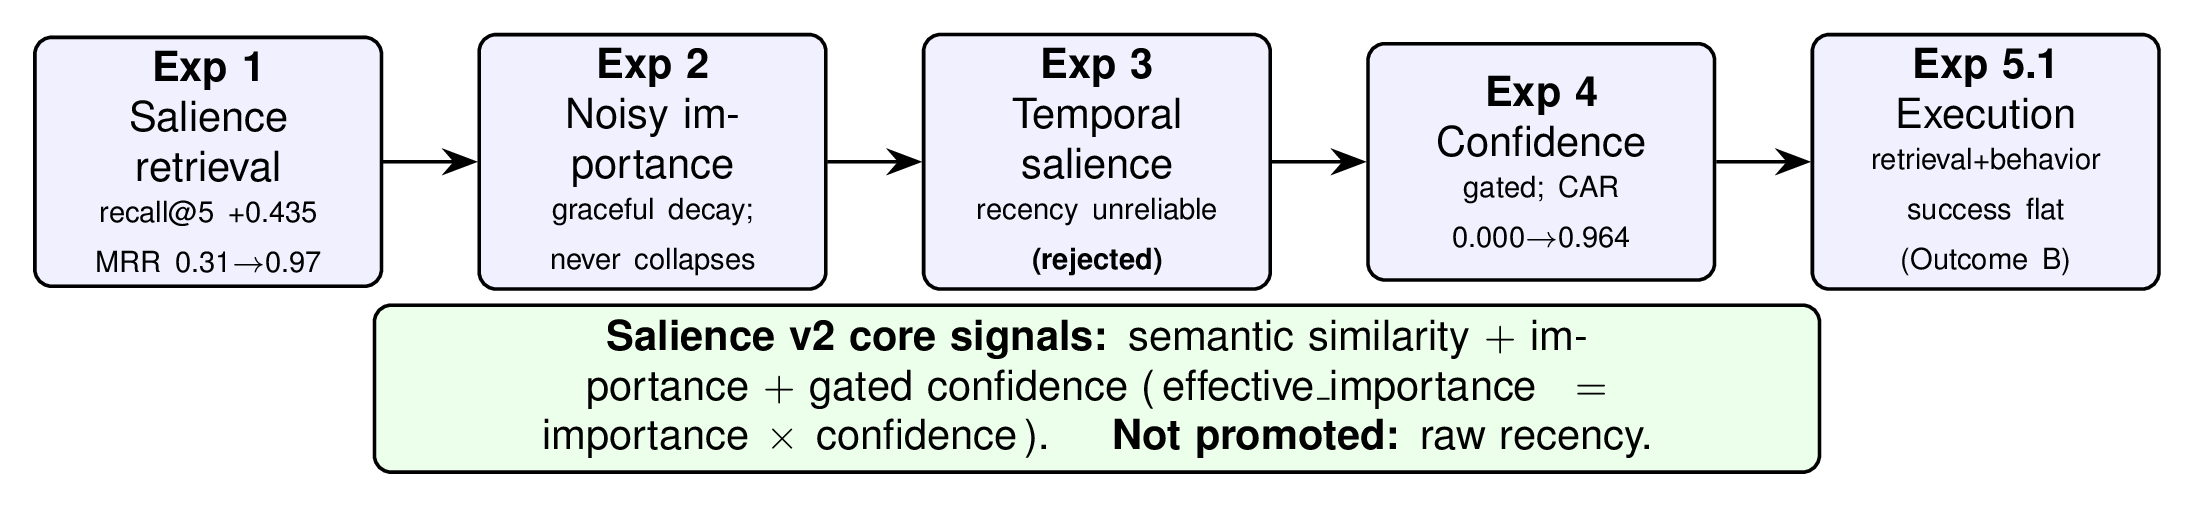
\includegraphics[width=0.9\textwidth]{figure10_program_overview.png}
\caption{Research program overview: the five experiments and how each probes a weakness of
the result before it.}
\label{fig:program}
\end{figure}

\bibliographystyle{plain}
\bibliography{refs}

\end{document}
